\documentclass[12pt]{article}   % artigo fonte 12
\usepackage[
a4paper,		% papel A4
left=1.5cm,		% margem esquerda
right=1.5cm,		% margem direita
top=1.5cm,		% margem superior
bottom=1.5cm		% margem inferior
]{geometry}
% Caracteres / Acentos / Português do Brasil
\usepackage[utf8]{inputenc}
\usepackage[T1]{fontenc}	
\usepackage[brazil]{babel}
% Pacotes Matemática
\usepackage{array,latexsym}
\usepackage{amsmath,amsfonts,amssymb,amsthm,mathabx,amstext}
\usepackage{dsfont}	% Conjuntos: $\mathds{N, Z, Q, R, C}$
\usepackage{graphicx}	
\begin{document}
	
	\begin{figure}[h!]
		
\includegraphics[scale=0.7]{ufpbde}
	\end{figure}
\par \textbf{Nome:} \underline{Paulo Ricardo Seganfredo Campana}
\par \textbf{Matricula:} \underline{20210044220}
\par \textbf{Nota:}
\vspace{+12pt}

\par \textbf{Questão 2}
	\begin{figure}[h!]
		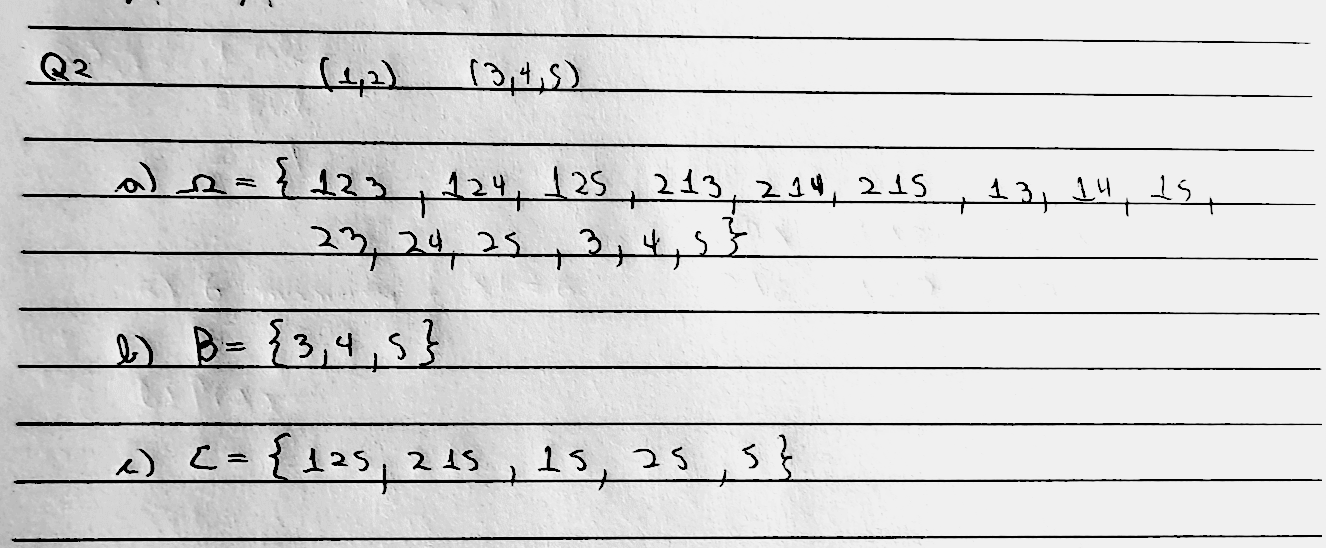
\includegraphics[scale=0.4]{q2}
	\end{figure}
\vspace{+12pt}
\par \textbf{Questão 8}
	\begin{figure}[h!]
		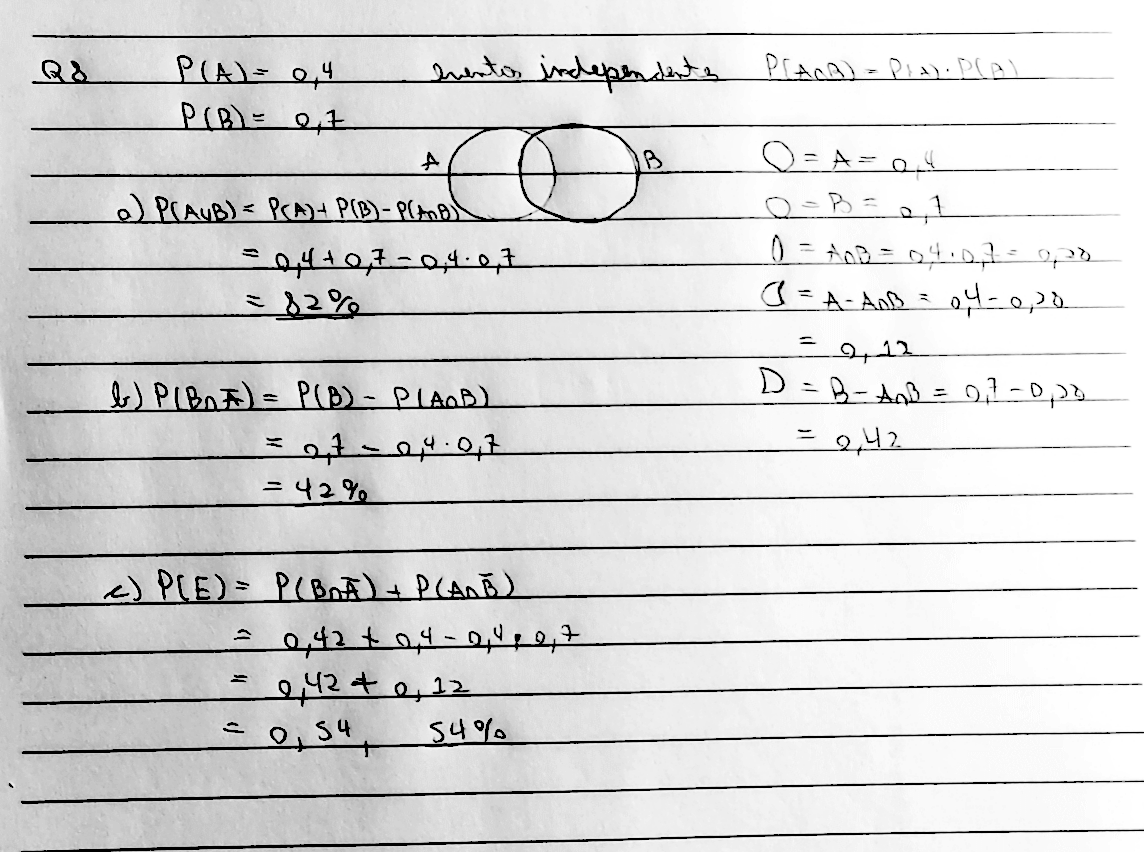
\includegraphics[scale=0.5]{q8}
	\end{figure}
\vspace{+12pt}

\par \textbf{Questão 12}
	\begin{figure}[h!]
		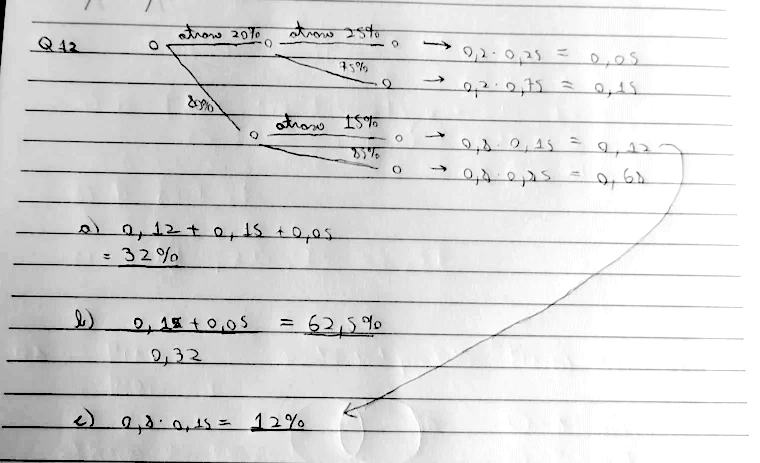
\includegraphics[scale=0.9]{q12}
	\end{figure}
\vspace{+12pt}

\par \textbf{Questão 18}
	\begin{figure}[h!]
		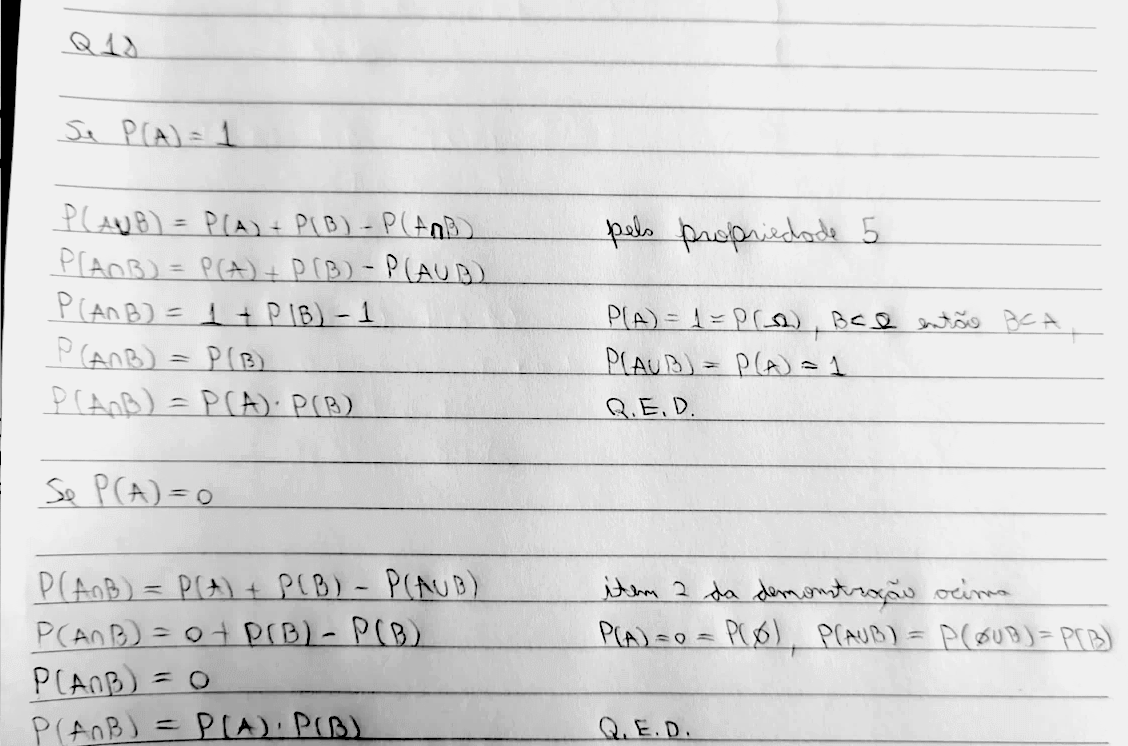
\includegraphics[scale=0.6]{q18}
	\end{figure} 	
\vspace{+12pt}




\end{document}